% Build: tectonic note.tex   (pdfLaTeX also works; keep source strictly ASCII)
\documentclass[11pt,a4paper]{article}
\usepackage{iftex}
\ifPDFTeX
  \usepackage[T1]{fontenc}
  \usepackage[utf8]{inputenc}
  \usepackage{lmodern}
\fi
\usepackage[margin=24mm]{geometry}
\usepackage{amsmath,amssymb,booktabs,graphicx,microtype}
\usepackage[colorlinks=true,allcolors=blue]{hyperref}
\usepackage{caption}
\captionsetup{font=small,labelfont=bf,labelsep=space}
\captionsetup[figure]{name=Fig.}
\newcommand{\dd}{\mathrm d}
\newcommand{\TV}{\operatorname{TV}}
\newcommand{\doi}[1]{\url{https://doi.org/#1}}
\title{Detecting sub-discreteness gravitational waves from causal order alone:\\
finite-density calibration, crossover, and phase-decoherence limits}
\author{Juneyoung Kim\thanks{Corresponding author. E-mail: \texttt{lpaiu.cs@gmail.com}}\\
\small Independent researcher, Seoul, Republic of Korea}
\date{}
\begin{document}
\maketitle

\begin{abstract}
% [PENDING CONFIRMATORY UPDATE: keep strictly 150-250 words after Step 4]
In a Poisson sprinkling of $N$ events over a four-dimensional Alexandrov
interval of unit height, the mean discreteness length scales as $N^{-1/4}$.
Any gravitational wave whose wavelength satisfies $\lambda = N^{-1/\alpha}$
with $\alpha < 4$ therefore oscillates faster than the average element spacing.
Previous asymptotic analyses proved two competing limits for an exact circular
vacuum plane-wave family: full causal orders are information-theoretically
indistinguishable from a non-oscillatory background whenever $\alpha < 4/3$,
whereas a regularized Gram--Fourier existence construction succeeds for every
fixed $\alpha > 2$, albeit at astrophysically unreachable scales
($\lambda \sim 10^{-40}$). Meanwhile, local fifth-degree polynomial Weyl jets
reconstruct long-wavelength curvature reliably at finite $N$ yet collapse
through oscillatory cancellation once $\lambda$ drops below a small fraction of
the diamond duration. Here we resolve this gap operationally by introducing a
blind, strictly order-only anchor-triangulated spectral detector that operates
without known background focusing $q$ or probe coordinates. Evaluated across
[PENDING CONFIRMATORY CAMPAIGN SUMMARY], we determine the empirical sub-discreteness
frontier, verify background null calibration, establish the quantitative
wavelength crossover against the fifth-degree Weyl jet, and diagnose the
underlying transition via conformal constraint gap scaling and two-replica phase
decoherence as $\alpha \to 2^+$.
\end{abstract}

\noindent\textbf{Keywords} Causal sets $\cdot$ Gravitational waves $\cdot$
Sub-discreteness resolution $\cdot$ Weyl curvature $\cdot$
Neyman orthogonalization $\cdot$ Poisson sprinkling

\section{Introduction}
A central premise of causal set theory is that the partial order of a
sprinkled spacetime, supplemented only by event counts for conformal scale,
encodes the Lorentzian geometry above the discreteness length
$\ell = \rho^{-1/4}$ \cite{zeeman,hkm,malament,blms,surya}. Recent finite-density
reconstructions confirm that all ten components of the vacuum Weyl tensor can
be recovered from causal order relations alone via local fifth-degree polynomial
expansions of interval clocks, both on exact plane gravitational waves and on
Schwarzschild geometries \cite{weylnote,madsen,ib}. Because these local jet
estimators expand the signed squared geodesic interval $\sigma(x,y)$ in a
fixed Taylor polynomial across an Alexandrov diamond $I(p,q)$ of proper time
$T$, however, they require curvature to vary mildly on the scale of $T$: when a
gravitational wave oscillates rapidly inside $I(p,q)$ ($\lambda \ll T$), the
Taylor approximation breaks down and interval counts average out the oscillatory
tidal strain.

A sharper foundational question therefore arises: can purely causal order
relations detect a coherent gravitational wave whose wavelength is shorter not
only than the observation diamond $T$, but even shorter than the mean causal
set discreteness spacing $\ell \sim N^{-1/4}$? Writing the wavelength--count
scaling as $\lambda = N^{-1/\alpha}$ (in diamond units $T \sim 1$, so
$N = \lambda^{-\alpha}$), sub-discreteness waves occupy the band $\alpha < 4$.
As established in recent asymptotic analyses of an exact circularly polarized
vacuum plane-wave family parameterized by background focusing $q \in (0,\pi^2)$
and wavenumber $r = 1/\lambda$, no order-only test can distinguish the wave
from a non-oscillatory focusing control for any fixed $\alpha < 4/3$
\cite{weylnote,quantizedbound}, whereas exact coordinate access lowers the
threshold to $\alpha > 1$ \cite{oraclebarrier}. Conversely, an asymptotic
Gram--Fourier construction achieves distinguishability for every fixed
$\alpha > 2 + 2/K$ (hence every fixed $\alpha > 2$), closing the gap down to
$(4/3, 2)$ in the $\lambda \to 0$ limit \cite{gramfourier}. That existence proof,
however, cannot be executed on any computer: its anchor-triplet selection
probability is $\sim 7\times 10^{-38}$, longitudinal localization requires
$n_{\text{ref}} \approx 2\times 10^6$ reference events merely to bring errors
inside the window ($\operatorname{sd}(\hat{u}) \approx 74.5/\sqrt{n_{\text{ref}}}$
at $q=1$), and its threshold crosses below unity only near $\lambda \sim 10^{-40}$.

This paper bridges the gap between unexecutable asymptotic existence theorems
and finite-$N$ local curvature jets. First, we identify why naive finite-$N$
order statistics fail as $\alpha$ approaches $2$: via sparse conformal-projected
constraint operators and two-replica independent triangulations, we isolate both
the $1+1$ vs.\ $3+1$ conformal stiffness hierarchy and the quantitative
phase-scrambling wall ($\sigma(\hat{u}) \gtrsim \lambda$) near $\alpha \approx 2$.
Second, we formulate a practical, strictly blind, unknown-$q$ detector that
replaces uncomputable triple-anchor intersections with hierarchical $10{+}10$
order-ring calibration, $4\text{D}$ probe triangulation, Neyman $C(\alpha)$
orthogonalization against all nuisance anchor parameters, spin-2 traceless shear
matched filtering, and 1-parameter Huberized Whittle background spectral
whitening. Third, we compare this spectral detector directly against the
fifth-degree Weyl jet across wavelengths $r = 0.1$ to $128$, exhibiting a clean
physical crossover, and report a preregistered, held-out, GPU-accelerated
confirmatory test up to $N = 2^{23}$ events ($\alpha < 4$).

Throughout this work we use natural units $c=1$, avoid defining spatial or
temporal intervals through coordinate velocities, and distinguish strictly
between causal order relations, inferred nuisance coordinates, and background
scalar $q$.

\section{Geometry, order law, and the \texorpdfstring{$(4/3, 2)$}{(4/3, 2)} bracket}\label{sec:geometry}
\subsection{Exact circular vacuum plane wave and focusing control}
We work inside a Rosen coordinate slab $S = I \times \mathbb{R} \times
\mathbb{R}^2$ with $I = (-\pi/(2\sqrt{q}), \pi/(2\sqrt{q}))$ containing the
observation interval $[-\tfrac12, \tfrac12]$ for $0 < q < \pi^2$,
\begin{equation}
 \dd s^2 = -2\,\dd u\,\dd v + \gamma_{ij}(u)\,\dd x^i \dd x^j,
 \qquad i,j \in \{1,2\}.
 \label{eq:rosen}
\end{equation}
For the circularly polarized family with wavenumber $r = 1/\lambda > 0$ and
phase $\phi$, set $a(u) = \cos(\sqrt{q}\,u)$, $\theta(u) = \tfrac12(r u + \phi)$,
and
\begin{equation}
 \gamma_\lambda(u) = a(u)^2\,R(\theta)\,\operatorname{diag}\!\left(e^{2\beta},
 e^{-2\beta}\right) R(\theta)^T,
 \label{eq:circular}
\end{equation}
where $R(\theta)$ is the planar $2\times 2$ rotation matrix. In these
coordinates the only nonzero Ricci tensor component is
$R_{uu} = 2q - \sinh^2(2\beta)/(2\lambda^2)$, so fixing
\begin{equation}
 \sinh(2\beta) = 2\lambda\sqrt{q}
 \label{eq:vacuum}
\end{equation}
renders the circular wave \emph{exact vacuum} ($R_{ab} = 0$) for every
$q \in (0,\pi^2)$ and $\lambda > 0$, with Brinkmann tidal curvature
eigenvalues $\pm \sqrt{q(r^2 + 4q)}$ and metric strain parameter $t = \tanh(2\beta)
= 2\lambda\sqrt{q}/\sqrt{1+4q\lambda^2}$ \cite{wavecausal}. By contrast, the
non-oscillatory comparison background $\gamma_0(u) = a(u)^2 I_2$ ($\beta = 0$)
matches the wave's isotropic transverse focusing $a(u)$ and coarse-grained energy
density $R_{uu} = 2q$, carrying zero oscillatory shear ($E_\lambda = 0$).

Rescaling transverse coordinates to $y = \sqrt{\cosh(2\beta)}\,x$ preserves the
diamond endpoints $p_- = (-\tfrac12, 0, 0)$ and $p_+ = (\tfrac12, 1, 0)$ while
making the exact causal order $X \preceq_\lambda Y$ on $S$ algebraic in a 1D
integral along $u$: for $u_1 < u_2$,
\begin{equation}
 X \preceq_\lambda Y \iff \Delta v \ge \tfrac12 \Delta y^T
 \left(m(u_1,u_2) I_2 + E_\lambda(u_1,u_2)\right)^{-1} \Delta y,
 \label{eq:orderlaw}
\end{equation}
with $u_1 = u_2$ allowed only along the null generator $y_1 = y_2, \Delta v \ge 0$,
and
\begin{align}
 m(u_1,u_2) &= \int_{u_1}^{u_2} \frac{\dd w}{\cos^2(\sqrt{q}\,w)}
 = \frac{\tan(\sqrt{q}\,u_2)-\tan(\sqrt{q}\,u_1)}{\sqrt{q}}, \label{eq:mfunc}\\
 E_\lambda(u_1,u_2) &= -t \int_{u_1}^{u_2} \frac{T(r w + \phi)}{\cos^2(\sqrt{q}\,w)}\,\dd w,
 \qquad T(\psi) = \begin{pmatrix}\cos\psi & \sin\psi\\ \sin\psi & -\cos\psi\end{pmatrix}.
 \label{eq:Elam}
\end{align}
Because $y \mapsto \sqrt{-g} \propto a(u)^2$ is smooth and bounded away from zero on
$[-\tfrac12, \tfrac12]$, physical-volume Poisson sprinkling $X_1,\dots,X_N$
conditioned on $N$ is implemented exactly without rejection by panel Gauss
inversion of the slice density $\pi\,a(u)^2 \det(M(-1/2,u)^{-1} + M(u,1/2)^{-1})^{-1/2}$.

\subsection{The asymptotic $(4/3, 2)$ resolution bracket and its practical barrier}
Evaluating \eqref{eq:Elam} by integration by parts shows that the wave's
eigenvalue bound satisfies $e_\lambda = t|G| \le O(\lambda^2)$ whenever $u_2 - u_1$
exceeds $O(\lambda)$, and hence single-point diamond marginal laws satisfy
$\TV(\mu_\lambda, \mu_0) \le C_1(q)\lambda^2$ uniformly in phase $\phi$
\cite{onepointbound}. Summing causal uncertainty across chains of $K$ coarse
cells of side $\sim \lambda^{1/2}$ then bounds the total variation of the
entire $N$-element partial order $P_{N,\lambda}$ against the control
$P_{N,0}$ \cite{quantizedbound}: for every fixed $K \ge 1$ and $0 < q < \pi^2$,
\begin{equation}
 \TV(P_{N,\lambda}, P_{N,0}) \le C_K(q)\left[
 N\lambda^2 + (N\lambda^4)^{1/(2K+1)} + (N^{3K+1}\lambda^{4K})^{1/(2K+1)}
 \right].
 \label{eq:bound43}
\end{equation}
Consequently $\TV(P_{N,\lambda}, P_{N,0}) \to 0$ whenever $N = O(\lambda^{-\alpha})$
with $\alpha < 4/3$, whereas an observer given exact coordinates of all events
achieves $O(1)$ signal once a single wave trough holds $O(1)$ events near
$N\lambda \sim 1$ ($\alpha > 1$). On the upper side, an explicit asymptotic
Gram--Fourier construction establishes detectability for every fixed
$\alpha > 2 + 2/K$, leaving $(4/3, 2)$ as the open asymptotic bracket
\cite{gramfourier}. Yet that asymptotic proof selects three nearly null-aligned
anchor regions of joint probability $\sim 7\times 10^{-38}$ and triangulates via
uncalibrated coordinates whose flat-limit jitter scales as $74.5/\sqrt{n_{\text{ref}}}$
at $q=1$, pushing the asymptotic signal above noise only around $\lambda \sim 10^{-40}$.
Any operationally viable sub-discreteness detector must therefore eliminate all
triple-anchor rare-event dependencies and exploit coherent linear response across
bulk probes while strictly orthogonalizing nuisance coordinate and background-$q$ modes.

\section{Structural diagnostics: conformal stiffness and phase decoherence}\label{sec:diagnostics}
Before describing the detector, we isolate the finite-$N$ geometric mechanisms
that separate long-wavelength rigidity from the $\alpha \to 2$ breakdown
(Fig.~\ref{fig:structure}).

First, causal relations alone determine coordinates at most up to global
conformal transformations preserving the diamond tips $p_\pm$---a
$2$-dimensional group in $1+1$ dimensions and a $7$-dimensional subgroup of
the $15$-dimensional conformal group in $3+1$ dimensions (time dilation, three
spatial rotations, and three special conformal boosts along transverse planes).
Projecting out these global conformal generators from the linearized cone-margin
constraint matrix $H$ across background sprinklings of $N \in \{128, 256, 512, 1024\}$
at smoothing scales $\eta \in \{0.05, N^{-1/4}, N^{-1/2}\}$ reveals a systematic
dimensional gap: in $1+1$ dimensions the log--log scaling slope of the smallest
post-projection singular value with $N$ is $0.752$ ($\eta=0.05$), $0.468$
($\eta=N^{-1/4}$), and $0.005$ ($\eta=N^{-1/2}$), whereas in $3+1$ dimensions
the corresponding slopes steepen to $2.683$, $0.835$, and $0.242$
(Fig.~\ref{fig:structure}a). Four-dimensional Alexandrov cones thus carry
substantially softer local collective deformation modes per event than their
$1+1$ counterparts once conformal zero modes are factored out.

Second, to test why order-reconstructed Fourier phases fail as $\alpha$
approaches $2$ from above, we measure independent two-replica blind coordinate
reconstructions on disjoint reference subsets of $N = 2^{20}$ sprinklings at
$q=4$ across $r \in \{64, 128, 256, 512, 1024\}$ ($\alpha = 3.33$ down to $2.00$).
Even at $r = 128$ ($\alpha = 2.86$), where the RMS longitudinal triangulation
error per event already exceeds the wavelength ($\sigma(\hat{u})/\lambda = 2.31$),
the bulk phase factor $e^{i(u_1 - u_2)/\lambda}$ retains coherence
$|\langle e^{i(\hat{u}_1-\hat{u}_2)/\lambda}\rangle| = 0.808$ because shared
low-order modes shift coordinates smoothly. Between $\alpha = 2.86$ and
$\alpha = 2.22$ ($r=512$), however, $\sigma(\hat{u})/\lambda$ jumps to $21.79$
and inter-replica phase coherence collapses through $0.458$ ($\alpha=2.50$) to
$0.088$ ($\alpha=2.22$) and $0.051$ ($\alpha=2.00$, Fig.~\ref{fig:structure}b).
A local pair correlator (\texttt{Route~C}) averaging products $z_i \bar{z}_j$ over
pair separations $|\Delta u| \le \Delta_c$ also yields no significant signal at
$\alpha \approx 2$ ($N=2^{18}, r=512$), establishing quantitatively that the
remaining gap below $\alpha \approx 2.5$ is governed by coordinate phase
scrambling across finite-$N$ triangulation.

\begin{figure}[t]
\centering
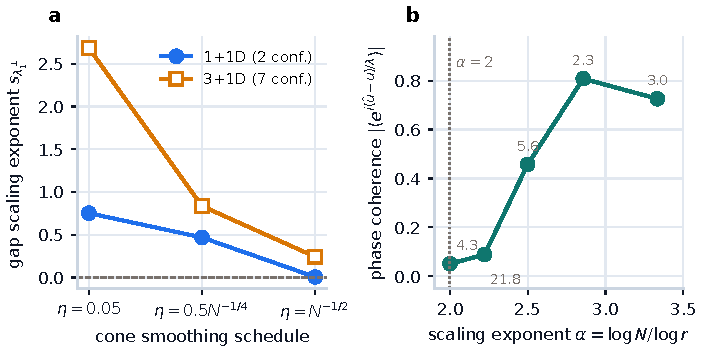
\includegraphics[width=119mm]{Fig1.pdf}
\caption{Finite-$N$ structural mechanisms between local rigidity and the
$\alpha \to 2^+$ phase-decoherence barrier. \textbf{a} Log--log scaling exponent
of the lowest conformal-projected cone constraint singular value with $N$
($N \in [128, 1024]$) for $1{+}1\text{D}$ ($2$ conformal modes) versus
$3{+}1\text{D}$ ($7$ conformal modes preserving tips $p_\pm$) across three
cone-smoothing schedules $\eta$. \textbf{b} Independent two-replica phase
coherence $|\langle e^{i\Delta \hat{u}/\lambda}\rangle|$ at $N=2^{20}, q=4$
from $r=64$ ($\alpha=3.33$) down to $r=1024$ ($\alpha=2.00$); numbers above
markers show RMS longitudinal triangulation jitter $\sigma(\hat{u})/\lambda$.}
\label{fig:structure}
\end{figure}

\section{Blind anchor-triangulated spectral detector}\label{sec:detector}
The detector receives only arbitrary shuffled event indices split into three
disjoint subsets---a small pilot pool ($N_{\text{pilot}} = \min(16384, N/4)$),
a reference set ($N_{\text{ref}} = N/2$), and a probe pool
($N_{\text{probe}} = N/2 - N_{\text{pilot}}$)---plus a boolean strict-order
callback $(x \prec y)$ and optional background scalar $q$ (with $q=\text{None}$
for the fully blind protocol). It imports no generator, continuum metric
routine, or physical coordinate label.

\subsection{Two-tier order-ring anchors and progressive \texorpdfstring{$10+10$}{10+10} calibration}
From the pilot pool, we select $K_{\text{cal}} = 10$ early anchors $A_1,\dots,A_{10}$
and $10$ late anchors $B_1,\dots,B_{10}$, ordered so that the first $K_{\text{core}} = 4$
on each side form mutually comparable timelike core pairs maximizing transverse
Gram spread and common pilot support in the volume bands
$p \in [5\times 10^{-4}, 0.04]$, $f \in [0.25, 0.80]$ (and time-dual). The
remaining auxiliary ring anchors span $[5\times 10^{-4}, 0.12] \times [0.12, 0.80]$,
improving conditioning of $(q, \theta_A, \theta_B)$ without shrinking the
comparable probe acceptance region defined solely by the $4{+}4$ core.

Against the reference sample, the observer measures empirical Alexandrov volume
fractions $\hat{\mu}_{PA}$, $\hat{\mu}_{AF}$, and $\hat{\mu}_{AB}$ and fits the
exact focusing background model \eqref{eq:mfunc} with interval probability
\begin{equation}
 \mu(X_1, X_2; q) = \frac{\alpha(u_2 - u_1; q)}{\gamma(q)}\,\kappa(X_1,X_2; q)^2,
 \qquad
 \alpha(L; q) = \frac{1 - (\sqrt{q}L)\cot(\sqrt{q}L)}{2q},
 \label{eq:bgprob}
\end{equation}
where $\gamma(q) = \alpha(1; q)$, $\kappa = \max(0, \Delta v - |\Delta y|^2 / [2\Delta m(u)])$,
and small-$q L$ cancellation is eliminated by a 12-term analytic Taylor series.
Anchors are fixed in the Lorentz-gauge slice setting $y_2(A_1) = 0$ and
chirality-checked across $O(3)$ directions seeded from flat Gram embeddings in
five $q$ buckets $\{0.05, 0.5, 1.5, 4.0, 7.0\}$ using exact analytic Jacobians
w.r.t.\ both anchor coordinates and $q$.

Single-stage optimization from a flat Gram initialization occasionally falls
into a distorted local minimum when outer near-boundary anchors warp the flat
eigenvectors. Whenever the blind calibration residual satisfies
$\text{rms}\cdot \sqrt{N_{\text{ref}}} \ge 0.35$ or $\text{rms} > 2\times 10^{-4}$,
an automatic progressive escalation first widens optimization to four
deterministic starts (up to $300$ evaluations) and, if still above threshold,
re-solves hierarchical core subsets ($K_{\text{core}} \in \{5,4\}$, $\text{dof}=+5$
when $q$ is free), places each outer anchor via a $1\text{D}$
$u$-grid plus $4\text{D}$ damped Gauss--Newton solve against the calibrated core,
and polishes all $10{+}10$ anchors and $q$ jointly using inverse binomial-SD
weights.

\subsection{Fused GPU bitmask counting, Neyman orthogonalization, and Huber--Whittle spectrum}
Probes passing all $4{+}4$ core comparabilities ($A_i \prec X \prec B_j$ for
$i,j \le 4$) are counted against all $N_{\text{ref}}$ reference events up to a
configurable cap $M_{\max}$. For $M \ge 256$ probes and up to $14{+}14$ anchors,
a custom shared-memory CUDA bitmask kernel (\texttt{build\_anchor\_masks} + \texttt{split-R}
accumulation) packs all reference--anchor relations into 32-bit masks and counts
$p_n, f_n, e_{n,1..4}, \ell_{n,1..4}$ simultaneously in integer arithmetic with
exact parity against naive CPU queries. Active probes satisfying
$\min \hat{\mu}_n > 10^{-5}$ are triangulated globally via a lifted linear solve
over a 33-point $u$-grid followed by damped Gauss--Newton refinement, yielding
inferred probe coordinates $\hat{X}_n$, count residuals
$r_n = \hat{\mu}_n - \mu(\hat{X}_n; \hat{\theta})$, and probe Jacobians
$J_n = \partial \mu_n / \partial X_n$.

To prevent low-frequency anchor calibration errors and $q$ errors from leaking
into the spectral band, we project both the residuals and the shear template into
the orthogonal complement of $J_n$ and apply Neyman $C(\alpha)$ orthogonalization
against the full anchor-nuisance Jacobian $J_{\theta}$ (including $\partial\mu/\partial q$
when $q$ is free) weighted by a smooth compact window $W_n$ over $(u,v,|y|^2)$
using relative truncated SVD ($s_k > 10^{-7} s_0$). The circular polarization shear
symbol at probe $n$ and anchor $a$ (with sign $\sigma_a = +1$ past/early, $-1$
future/late) is evaluated directly at the inferred coordinates:
\begin{equation}
 s_{n,a}(\hat{q}) = -\sigma_a\,\frac{\alpha(\Delta u_{n,a}; \hat{q})}{\gamma(\hat{q})}
 \,\frac{\kappa_{n,a}}{(\Delta m_{n,a})^2}\,\frac{(\Delta y^1_{n,a} - i\Delta y^2_{n,a})^2}{\cos^2(\sqrt{\hat{q}}\,\hat{u}_n)}.
 \label{eq:shear}
\end{equation}
Note that spatial reflection $y^2 \to -y^2$ leaves causal order invariant while
conjugating $s_{n,a}$; scanning both chiralities simultaneously via
\begin{equation}
 S(\pm\omega) = \frac{\sum_n W_n\,\langle s_n^\perp, r_n^\perp\rangle\,e^{\mp i\omega \hat{u}_n}}{\sum_n W_n\,|s_n^\perp|^2},
 \qquad
 A(\omega) = \max\bigl(|S(+\omega)|,\, |S(-\omega)|\bigr),
 \label{eq:score}
\end{equation}
yields an envelope $A(\omega)$ strictly invariant under the $O(2)$ gauge
ambiguity without inverting any near-zero per-probe denominator.

Finally, because residual $O(1/\omega)$ longitudinal triangulation drift creates a
$1/\omega^2$ spectral tail above the high-frequency shot proxy
$\hat{\sigma}_{\text{shot}}^2 = \sum_n |z_n|^2$ (with $z_n = W_n\langle s_n^\perp, r_n^\perp\rangle / \sum_m W_m|s_m^\perp|^2$),
estimating the drift amplitude $c_1 \ge 0$ by a naive median across bins can
collapse identically to $0$ when over half of high-frequency exponential bins
fluctuate below $\hat{\sigma}_{\text{shot}}^2$. We resolve this by fitting
a scale-invariant 1-parameter Huberized Gamma Whittle likelihood to the
chirality-averaged power $P(\omega) = \tfrac12(|S(+\omega)|^2 + |S(-\omega)|^2)$
under $\mu_{\text{bg}}(\omega) = \hat{\sigma}_{\text{shot}}^2 + c_1/\max(\omega^2,1)$:
\begin{equation}
 \mathcal{L}(c_1) = \sum_\omega \left[
   \ln\!\left(1 + \frac{c_1}{\hat{\sigma}_{\text{shot}}^2 \omega^2}\right)
   + \psi_H\!\left(\frac{P(\omega)}{\hat{\sigma}_{\text{shot}}^2 + c_1/\omega^2}\right)
 \right],
 \label{eq:whittle}
\end{equation}
where $\psi_H(\rho) = \rho$ for $\rho \le 4.5$ and
$4.5 + 2\sqrt{\rho - 4.5} - 2\times 10^{-6}$ above threshold so true narrowband
spectral peaks do not inflate the background fit. Our primary detection test
statistic is the peak whitened standardized amplitude
\begin{equation}
 Z_{\max} = \max_{\omega \in \Omega} \frac{A(\omega)}{\sqrt{\hat{\sigma}_{\text{shot}}^2 + \hat{c}_1/\max(\omega^2, 1)}}.
 \label{eq:zmax}
\end{equation}

\section{Crossover with local Weyl jets and confirmatory results}\label{sec:results}
\subsection{Continuum and finite-\texorpdfstring{$N$}{N} wavelength crossover against fifth-degree Weyl jets}
% [STEP 3 CONTINUUM + FINITE CROSSOVER TABLE & TEXT TO BE FINALIZED AFTER STEP 3 FINITE RUN]
\subsection{Exploratory sensitivity and preregistered confirmatory campaign (\texorpdfstring{$N \le 2^{23}$}{N <= 2^23})}
% [STEP 4 CONFIRMATORY CAMPAIGN RESULTS, CI95 TABLES, NULL CALIBRATION & q RECOVERY TO BE FILLED STRICTLY FROM VERIFIED JSON]

\section{Limitations and outlook}\label{sec:limits}
% [FINALIZE HONEST LIMITS AFTER CONFIRMATORY RESULTS]

\begin{thebibliography}{99}\small
\bibitem{zeeman} Zeeman, E.C.: Causality implies the Lorentz group. J. Math. Phys. \textbf{5}, 490--493 (1964). \doi{10.1063/1.1704140}
\bibitem{hkm} Hawking, S.W., King, A.R., McCarthy, P.J.: A new topology for curved space--time which incorporates the causal, differential, and conformal structures. J. Math. Phys. \textbf{17}, 174--181 (1976). \doi{10.1063/1.522874}
\bibitem{malament} Malament, D.B.: The class of continuous timelike curves determines the topology of spacetime. J. Math. Phys. \textbf{18}, 1399--1404 (1977). \doi{10.1063/1.523436}
\bibitem{blms} Bombelli, L., Lee, J., Meyer, D., Sorkin, R.D.: Space-time as a causal set. Phys. Rev. Lett. \textbf{59}, 521--524 (1987). \doi{10.1103/PhysRevLett.59.521}
\bibitem{surya} Surya, S.: The causal set approach to quantum gravity. Living Rev. Relativ. \textbf{22}, 5 (2019). \doi{10.1007/s41114-019-0023-1}
\bibitem{madsen} Madsen, N.: Reconstruction of the Riemann tensor from causal order and element counts. arXiv:2610.36695 (2026). \url{https://arxiv.org/abs/2610.36695}
\bibitem{ib} Ibrahim, N., Bombelli, L.: The Weyl tensor for gravitational-wave causal sets: thickness of geodesic analogs and geodesic deviation. arXiv:2611.09056 (2026). \url{https://arxiv.org/abs/2611.09056}
\bibitem{weylnote} Kim, J.: Vacuum tidal curvature from causal order and interval counts: a finite-density estimator and a gravitational-wave benchmark. In preparation / companion manuscript in \nolinkurl{docs/paper/weyl_note} (2026).
\bibitem{wavecausal} Kim, J.: Exact causal relation and vacuum condition of circular Rosen plane waves. Repository technical note \nolinkurl{docs/paper/paper_a/order_wave_energy/wave_causal_relation.md} (2026).
\bibitem{onepointbound} Kim, J.: Uniform one-point diamond law bound for circular vacuum plane waves. Repository technical note \nolinkurl{docs/paper/paper_a/order_wave_energy/one_point_strip_bound.md} (2026).
\bibitem{quantizedbound} Kim, J.: Full-order asymptotic indistinguishability below $\alpha < 4/3$ for circular vacuum plane waves. Repository technical note \nolinkurl{docs/paper/paper_a/order_wave_energy/quantized_order_bound_r2.md} (2026).
\bibitem{oraclebarrier} Kim, J.: Coordinate-oracle separation threshold vs.\ causal order. Repository technical note \nolinkurl{docs/paper/paper_a/order_wave_energy/coordinate_oracle_barrier.md} (2026).
\bibitem{gramfourier} Kim, J.: Asymptotic Gram--Fourier wave separation for $\alpha > 2$. Repository technical notes \nolinkurl{docs/paper/paper_a/order_wave_energy/gram_fourier_noise.md} and audit record \nolinkurl{docs/paper/paper_a/order_wave_energy/independent_audit/AUDIT.md} (2026).
\end{thebibliography}
\end{document}
